\chapter{Introduzione}

In questo capitolo vengono introdotti i concetti base delle Interfacce Uomo-Macchina. Il corso esplora come l'uomo interagisce con i sistemi informatici e viceversa, comprese le componenti fisiche (segnali corporei) e gli algoritmi (Machine Learning) usati per dare un senso a questi dati.

\section{Ciclo di Interazione}

Di seguito uno schema generale dell'interazione Uomo-Macchina:

\begin{figure}[h!]
    \centering
    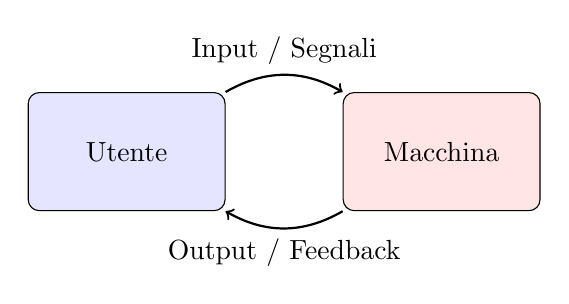
\begin{tikzpicture}[node distance=4cm, auto]
        \node[draw, rectangle, rounded corners, minimum height=1.5cm, minimum width=2.5cm, fill=blue!10] (human) {Utente};
        \node[draw, rectangle, rounded corners, minimum height=1.5cm, minimum width=2.5cm, fill=red!10, right of=human] (machine) {Macchina};

        \draw[->, thick] (human.north east) to[bend left] node[midway, above] {Input / Segnali} (machine.north west);
        \draw[->, thick] (machine.south west) to[bend left] node[midway, below] {Output / Feedback} (human.south east);
    \end{tikzpicture}
    \caption{Schema del ciclo base di interazione tra uomo e macchina.}
\end{figure}

\section{Evoluzione Storica delle Interfacce}
L'interazione uomo-macchina ha subito profonde trasformazioni nel corso dei decenni. Possiamo riassumere questa evoluzione in 5 fasi principali:
\begin{itemize}
    \item \textbf{Manuale (Batch):} Interazione indiretta tramite schede perforate e interruttori fisici.
    \item \textbf{Riga di Comando (CLI):} Interazione basata su testo, richiede conoscenza di sintassi e comandi specifici.
    \item \textbf{Interfacce Grafiche (GUI):} Introduzione del paradigma WIMP (Window, Icon, Menu, Pointer), rendendo l'uso accessibile alla massa.
    \item \textbf{Web e Mobile:} Interfacce touch, navigazione ipertestuale e proliferazione sugli smartphone.
    \item \textbf{Interfacce Multimodali e Intelligenti:} Interazioni naturali sfruttando voce, gesti e adattabilità del sistema (HCI moderna).
\end{itemize}

\section{Multimodalità vs Multimedialità}
È fondamentale distinguere tra concetti spesso confusi:
\begin{itemize}
    \item \textbf{Multimedialità:} Si riferisce al sistema che comunica \emph{all'utente} attraverso diversi tipi di media (testo, audio, video). Riguarda principalmente l'output.
    \item \textbf{Multimodalità:} Riguarda le modalità con cui l'utente fornisce input \emph{alla macchina}. Un'interfaccia multimodale permette l'uso congiunto e sinergico di diversi canali, come:
    \begin{itemize}
        \item \textbf{Voce e Parola} (es. Speech Recognition)
        \item \textbf{Gesti e Postura}
        \item \textbf{Eye-tracking} (tracciamento oculare)
        \item \textbf{Segnali Fisiologici} (HR, EDA, EEG)
    \end{itemize}
\end{itemize}

\section{Applicazioni Reali}
Le moderne HMI (Human-Machine Interfaces) trovano applicazione in contesti complessi e critici:
\begin{itemize}
    \item \textbf{Realtà Virtuale (VR) e Aumentata (AR):} Utilizzate per simulazioni o supporto (es. torri di controllo aereo con interfacce aumentate per gestire alti flussi di dati visivi in modo efficiente).
    \item \textbf{Social Robots:} Robot impiegati come compagni per anziani o per supporto terapeutico, dotati di capacità di comprensione delle emozioni (Affective Computing).
    \item \textbf{Sistemi Assisistivi alla Guida (ADAS):} Rilevamento dello stato psicofisico del guidatore (stress, sonnolenza, fatica alla guida) misurando parametri corporei e comportamento oculare per prevenire incidenti.
    \item \textbf{Tecnologie Assistive:} Applicazioni cliniche per soggetti con gravi disabilità motorie (es. SLA), come esoscheletri robotici controllati da segnali muscolari/cerebrali, e sistemi di Brain-Computer Interface (BCI).
\end{itemize}
